% Options for packages loaded elsewhere
\PassOptionsToPackage{unicode}{hyperref}
\PassOptionsToPackage{hyphens}{url}
%
\documentclass[
  12 pt,
  a4paper,
]{article}
\usepackage{amsmath,amssymb}
\usepackage{setspace}
\usepackage{iftex}
\ifPDFTeX
  \usepackage[T1]{fontenc}
  \usepackage[utf8]{inputenc}
  \usepackage{textcomp} % provide euro and other symbols
\else % if luatex or xetex
  \usepackage{unicode-math} % this also loads fontspec
  \defaultfontfeatures{Scale=MatchLowercase}
  \defaultfontfeatures[\rmfamily]{Ligatures=TeX,Scale=1}
\fi
\usepackage{lmodern}
\ifPDFTeX\else
  % xetex/luatex font selection
  \setmainfont[]{Times New Roman}
\fi
% Use upquote if available, for straight quotes in verbatim environments
\IfFileExists{upquote.sty}{\usepackage{upquote}}{}
\IfFileExists{microtype.sty}{% use microtype if available
  \usepackage[]{microtype}
  \UseMicrotypeSet[protrusion]{basicmath} % disable protrusion for tt fonts
}{}
\makeatletter
\@ifundefined{KOMAClassName}{% if non-KOMA class
  \IfFileExists{parskip.sty}{%
    \usepackage{parskip}
  }{% else
    \setlength{\parindent}{0pt}
    \setlength{\parskip}{6pt plus 2pt minus 1pt}}
}{% if KOMA class
  \KOMAoptions{parskip=half}}
\makeatother
\usepackage{xcolor}
\usepackage[margin=1in]{geometry}
\usepackage{color}
\usepackage{fancyvrb}
\newcommand{\VerbBar}{|}
\newcommand{\VERB}{\Verb[commandchars=\\\{\}]}
\DefineVerbatimEnvironment{Highlighting}{Verbatim}{commandchars=\\\{\}}
% Add ',fontsize=\small' for more characters per line
\usepackage{framed}
\definecolor{shadecolor}{RGB}{248,248,248}
\newenvironment{Shaded}{\begin{snugshade}}{\end{snugshade}}
\newcommand{\AlertTok}[1]{\textcolor[rgb]{0.94,0.16,0.16}{#1}}
\newcommand{\AnnotationTok}[1]{\textcolor[rgb]{0.56,0.35,0.01}{\textbf{\textit{#1}}}}
\newcommand{\AttributeTok}[1]{\textcolor[rgb]{0.13,0.29,0.53}{#1}}
\newcommand{\BaseNTok}[1]{\textcolor[rgb]{0.00,0.00,0.81}{#1}}
\newcommand{\BuiltInTok}[1]{#1}
\newcommand{\CharTok}[1]{\textcolor[rgb]{0.31,0.60,0.02}{#1}}
\newcommand{\CommentTok}[1]{\textcolor[rgb]{0.56,0.35,0.01}{\textit{#1}}}
\newcommand{\CommentVarTok}[1]{\textcolor[rgb]{0.56,0.35,0.01}{\textbf{\textit{#1}}}}
\newcommand{\ConstantTok}[1]{\textcolor[rgb]{0.56,0.35,0.01}{#1}}
\newcommand{\ControlFlowTok}[1]{\textcolor[rgb]{0.13,0.29,0.53}{\textbf{#1}}}
\newcommand{\DataTypeTok}[1]{\textcolor[rgb]{0.13,0.29,0.53}{#1}}
\newcommand{\DecValTok}[1]{\textcolor[rgb]{0.00,0.00,0.81}{#1}}
\newcommand{\DocumentationTok}[1]{\textcolor[rgb]{0.56,0.35,0.01}{\textbf{\textit{#1}}}}
\newcommand{\ErrorTok}[1]{\textcolor[rgb]{0.64,0.00,0.00}{\textbf{#1}}}
\newcommand{\ExtensionTok}[1]{#1}
\newcommand{\FloatTok}[1]{\textcolor[rgb]{0.00,0.00,0.81}{#1}}
\newcommand{\FunctionTok}[1]{\textcolor[rgb]{0.13,0.29,0.53}{\textbf{#1}}}
\newcommand{\ImportTok}[1]{#1}
\newcommand{\InformationTok}[1]{\textcolor[rgb]{0.56,0.35,0.01}{\textbf{\textit{#1}}}}
\newcommand{\KeywordTok}[1]{\textcolor[rgb]{0.13,0.29,0.53}{\textbf{#1}}}
\newcommand{\NormalTok}[1]{#1}
\newcommand{\OperatorTok}[1]{\textcolor[rgb]{0.81,0.36,0.00}{\textbf{#1}}}
\newcommand{\OtherTok}[1]{\textcolor[rgb]{0.56,0.35,0.01}{#1}}
\newcommand{\PreprocessorTok}[1]{\textcolor[rgb]{0.56,0.35,0.01}{\textit{#1}}}
\newcommand{\RegionMarkerTok}[1]{#1}
\newcommand{\SpecialCharTok}[1]{\textcolor[rgb]{0.81,0.36,0.00}{\textbf{#1}}}
\newcommand{\SpecialStringTok}[1]{\textcolor[rgb]{0.31,0.60,0.02}{#1}}
\newcommand{\StringTok}[1]{\textcolor[rgb]{0.31,0.60,0.02}{#1}}
\newcommand{\VariableTok}[1]{\textcolor[rgb]{0.00,0.00,0.00}{#1}}
\newcommand{\VerbatimStringTok}[1]{\textcolor[rgb]{0.31,0.60,0.02}{#1}}
\newcommand{\WarningTok}[1]{\textcolor[rgb]{0.56,0.35,0.01}{\textbf{\textit{#1}}}}
\usepackage{longtable,booktabs,array}
\usepackage{calc} % for calculating minipage widths
% Correct order of tables after \paragraph or \subparagraph
\usepackage{etoolbox}
\makeatletter
\patchcmd\longtable{\par}{\if@noskipsec\mbox{}\fi\par}{}{}
\makeatother
% Allow footnotes in longtable head/foot
\IfFileExists{footnotehyper.sty}{\usepackage{footnotehyper}}{\usepackage{footnote}}
\makesavenoteenv{longtable}
\usepackage{graphicx}
\makeatletter
\def\maxwidth{\ifdim\Gin@nat@width>\linewidth\linewidth\else\Gin@nat@width\fi}
\def\maxheight{\ifdim\Gin@nat@height>\textheight\textheight\else\Gin@nat@height\fi}
\makeatother
% Scale images if necessary, so that they will not overflow the page
% margins by default, and it is still possible to overwrite the defaults
% using explicit options in \includegraphics[width, height, ...]{}
\setkeys{Gin}{width=\maxwidth,height=\maxheight,keepaspectratio}
% Set default figure placement to htbp
\makeatletter
\def\fps@figure{htbp}
\makeatother
\setlength{\emergencystretch}{3em} % prevent overfull lines
\providecommand{\tightlist}{%
  \setlength{\itemsep}{0pt}\setlength{\parskip}{0pt}}
\setcounter{secnumdepth}{-\maxdimen} % remove section numbering
\ifLuaTeX
\usepackage[bidi=basic]{babel}
\else
\usepackage[bidi=default]{babel}
\fi
\babelprovide[main,import]{spanish}
\ifPDFTeX
\else
\babelfont{rm}[]{Times New Roman}
\fi
% get rid of language-specific shorthands (see #6817):
\let\LanguageShortHands\languageshorthands
\def\languageshorthands#1{}
\ifLuaTeX
  \usepackage{selnolig}  % disable illegal ligatures
\fi
\usepackage{bookmark}
\IfFileExists{xurl.sty}{\usepackage{xurl}}{} % add URL line breaks if available
\urlstyle{same}
\hypersetup{
  pdfauthor={Tomàs Ferrandis Moscardó},
  pdflang={es-ES},
  hidelinks,
  pdfcreator={LaTeX via pandoc}}

\title{ANÁLISIS BIVARIADO SOBRE LIBERTADES EN ITALIA\\
Encuesta Social Europea, 2020/2022 (Ronda 10)}
\usepackage{etoolbox}
\makeatletter
\providecommand{\subtitle}[1]{% add subtitle to \maketitle
  \apptocmd{\@title}{\par {\large #1 \par}}{}{}
}
\makeatother
\subtitle{Técnicas de Investigación en Ciencia Política I. UBU\\
Práctica 2.}
\author{Tomàs Ferrandis Moscardó}
\date{2024-05-19}

\begin{document}
\maketitle

{
\setcounter{tocdepth}{2}
\tableofcontents
}
\setstretch{1.5}
\newpage
\renewcommand\tablename{Tabla}

\section{1 INTRODUCCIÓN}\label{introducciuxf3n}

\subsection{1.1 DESCRIPCIÓN DE LA
PRÁCTICA}\label{descripciuxf3n-de-la-pruxe1ctica}

Este trabajo versará sobre las libertades en Italia a partir de diversos
\textbf{análisis bivariados} sobre datos de la Encuesta Social Europea
de los años 2020 y 2022 ( Ronda 10). Se escogerá en cada caso el test
más adecuado y, finalmente, se hará una valoración crítica a partir de
los datos analizados. Las variables que se estudiarán en las siguientes
actividades corresponden al cuestionario de la encuesta.

La práctica está relacionada con los temas 5 y 6 de la asignatura
Técnicas de la Investigación en Ciencia Política I del Grado
Universitario de Ciencia Política y Gestión Pública de la Universidad de
Burgos, curso 2023-2024.

\subsection{1.2 LIBRERÍAS R}\label{libreruxedas-r}

Un primer paso será asegurar que en nuestra instalación de R están
disponibles algunas funciones necesarias para abrir el fichero de datos
externo (tipo .sav), para algún cálculo estadístico o formateo de datos
en Rmd.

\begin{Shaded}
\begin{Highlighting}[]
\ControlFlowTok{if}\NormalTok{(}\SpecialCharTok{!}\FunctionTok{require}\NormalTok{(haven))\{}\FunctionTok{install.packages}\NormalTok{(}\StringTok{"haven"}\NormalTok{)\} }\CommentTok{\# para abrir fichero .sav}
\FunctionTok{library}\NormalTok{(haven)}
\ControlFlowTok{if}\NormalTok{(}\SpecialCharTok{!}\FunctionTok{require}\NormalTok{(knitr))\{}\FunctionTok{install.packages}\NormalTok{(}\StringTok{"knitr"}\NormalTok{)\} }\CommentTok{\# Act. 2. Tabla Rd}
\FunctionTok{library}\NormalTok{(knitr)}
\ControlFlowTok{if}\NormalTok{(}\SpecialCharTok{!}\FunctionTok{require}\NormalTok{(DescTools))\{}\FunctionTok{install.packages}\NormalTok{(}\StringTok{"DescTools"}\NormalTok{)\} }\CommentTok{\#actividad 3}
\FunctionTok{library}\NormalTok{(DescTools)}
\ControlFlowTok{if}\NormalTok{ (}\SpecialCharTok{!}\FunctionTok{require}\NormalTok{(epiDisplay))\{}\FunctionTok{install.packages}\NormalTok{(}\StringTok{"epiDisplay"}\NormalTok{)\}}
\FunctionTok{library}\NormalTok{(epiDisplay)}
\ControlFlowTok{if}\NormalTok{ (}\SpecialCharTok{!}\FunctionTok{require}\NormalTok{(DescTools))\{}\FunctionTok{install.packages}\NormalTok{(}\StringTok{"DescTools"}\NormalTok{)\}}
\FunctionTok{library}\NormalTok{(DescTools)}
\end{Highlighting}
\end{Shaded}

\subsection{1.3 GESTIÓN DE FICHEROS Y CREACIÓN DE LA BASE DE
DATOS}\label{gestiuxf3n-de-ficheros-y-creaciuxf3n-de-la-base-de-datos}

\textbf{Ficheros externos}

Los datos se obtienen del fichero de los datos de la Encuesta Social
Europea (\emph{datosprac2.sav}). Este como cualquier fichero de
resultados se ubicarán en una subcarpeta DATOS del directorio donde se
esté este mismo fichero Rmd.

\begin{Shaded}
\begin{Highlighting}[]
\CommentTok{\# El fichero .sav debe estar en una subcarpeta DATOS}
\NormalTok{nombreFichero}\OtherTok{\textless{}{-}}\StringTok{"datosprac2.sav"}
\NormalTok{directorioTrabajo}\OtherTok{\textless{}{-}}\FunctionTok{getwd}\NormalTok{()}
\NormalTok{rutaFichero}\OtherTok{\textless{}{-}}\FunctionTok{paste}\NormalTok{(directorioTrabajo,}\StringTok{"DATOS"}\NormalTok{,nombreFichero,}\AttributeTok{sep=}\StringTok{"/"}\NormalTok{)}
\end{Highlighting}
\end{Shaded}

\textbf{Creación de la vbase de datos}

A partir del fichero de tipo sav (\textbf{datosprac2.sav}) de la
Encuesta Social Europea, se creará el \emph{data frame} de R. Esta será
la \textbf{base de datos} inicial con todos los datos de la encuesta.

\begin{Shaded}
\begin{Highlighting}[]
\NormalTok{df\_ronda10}\OtherTok{\textless{}{-}}\FunctionTok{read\_sav}\NormalTok{(rutaFichero)}
\end{Highlighting}
\end{Shaded}

\newpage

\section{2 ACTIVIDAD 1. CONTRASTE DE MEDIAS PARA DATOS
RELACIONADOS.}\label{actividad-1.-contraste-de-medias-para-datos-relacionados.}

\subsection{2.1 DESCRIPCIÓN DE LA ACTIVIDAD
1}\label{descripciuxf3n-de-la-actividad-1}

En esta primera actividad se realizará un contraste de hipótesis para
ver si dos variables presentan diferencias estadísticamente
significativas entre si.

Las variables son:

\begin{itemize}
\tightlist
\item
  \textbf{fairelcc: Las elecciones son libres y limpias en Italia}
  (Pregunta B3 del cuestionario).
\item
  \textbf{cttresac: Los tribunales en Italia tratan a todo el mundo por
  igual} (Pregunta B18 del cuestionario).
\end{itemize}

Ambas son Variables cualitativas ordinarias y admiten un valor que va
desde 0 (``No es válida en absoluto'') a 10 (``Es completamente
válido'') además de los valores considerados como no válidos a efectos
estadísticos 77, 88 y 99 (``Rechaza responder'', ``NS No sabe'' y ``NC
No contesta'' respectivamente).

\subsection{2.2 PREPARACIÓN DE LA BASE DE
DATOS}\label{preparaciuxf3n-de-la-base-de-datos}

\textbf{Recodificación de valores no válidos}

Se comprueba si hay valores que necesitan recodificarse. Serían los
valores externos al intervalo {[}0-10{]} que según el codebook de la
encuesta podrían ser 77, 88 ó 99 ya explicados.

\begin{Shaded}
\begin{Highlighting}[]
\FunctionTok{unique}\NormalTok{(df\_ronda10}\SpecialCharTok{$}\NormalTok{fairelcc)}
\end{Highlighting}
\end{Shaded}

\begin{verbatim}
##  [1]  7  6  2  5  8  1  0  3  9  4 NA 10
\end{verbatim}

\begin{Shaded}
\begin{Highlighting}[]
\FunctionTok{unique}\NormalTok{(df\_ronda10}\SpecialCharTok{$}\NormalTok{cttresac)}
\end{Highlighting}
\end{Shaded}

\begin{verbatim}
##  [1]  1  0  2  8  3  7  6  5  9  4 NA 10
\end{verbatim}

Se comprueba que ya deben estar recodificados o almenos no aparecen. No
obstante, en caso de que no fuese así, se procedería de la siguiente
manera.

\begin{itemize}
\tightlist
\item
  En primer lugar, se duplicarán los campos para hacer las modificación
  sobre estos.
\end{itemize}

\begin{Shaded}
\begin{Highlighting}[]
\NormalTok{df\_ronda10}\SpecialCharTok{$}\NormalTok{rec\_cttresac }\OtherTok{\textless{}{-}}\NormalTok{ df\_ronda10}\SpecialCharTok{$}\NormalTok{cttresac}
\NormalTok{df\_ronda10}\SpecialCharTok{$}\NormalTok{rec\_fairelecc }\OtherTok{\textless{}{-}}\NormalTok{df\_ronda10}\SpecialCharTok{$}\NormalTok{fairelcc}
\end{Highlighting}
\end{Shaded}

\begin{itemize}
\tightlist
\item
  Después, se recodifican los valores 77, 88 y 99 como NA
\end{itemize}

\begin{Shaded}
\begin{Highlighting}[]
\NormalTok{df\_ronda10}\SpecialCharTok{$}\NormalTok{rec\_fairelecc[df\_ronda10}\SpecialCharTok{$}\NormalTok{rec\_fairelecc }\SpecialCharTok{\textgreater{}=}\DecValTok{77} \SpecialCharTok{\&} 
\NormalTok{                            df\_ronda10}\SpecialCharTok{$}\NormalTok{rec\_fairelecc }\SpecialCharTok{\textless{}=}\DecValTok{99}\NormalTok{]}\OtherTok{\textless{}{-}}\ConstantTok{NA}

\NormalTok{df\_ronda10}\SpecialCharTok{$}\NormalTok{rec\_cttresac[df\_ronda10}\SpecialCharTok{$}\NormalTok{rec\_cttresac }\SpecialCharTok{\textgreater{}=}\DecValTok{77} \SpecialCharTok{\&} 
\NormalTok{                            df\_ronda10}\SpecialCharTok{$}\NormalTok{rec\_cttresac }\SpecialCharTok{\textless{}=}\DecValTok{99}\NormalTok{]}\OtherTok{\textless{}{-}}\ConstantTok{NA}
\end{Highlighting}
\end{Shaded}

\subsection{2.3 HIPÓTESIS}\label{hipuxf3tesis}

\begin{itemize}
\tightlist
\item
  Se plantea como \textbf{hipótesis nula (H0) que ambas medias son
  iguales}.
\item
  La hipótesis alternativa (H1) sería, por lo tanto, que las medias son
  distintas.
\end{itemize}

\subsection{2.4 PRUEBA DE T-STUDENT}\label{prueba-de-t-student}

Aplicaremos la función que implementa el método T-Student sobre los
campos duplicados en nuestro caso.

\begin{itemize}
\item
  \emph{paired = T}, indica a la función que operará con 2 muestras
  emparejadas.
\item
  \emph{alternative = `two.sized'}, indica que la hipótesis alternativa
  es que las medias no son iguales.
\item
  Se establece un \emph{nivel de confianza} del 95\%.
\end{itemize}

\begin{Shaded}
\begin{Highlighting}[]
\FunctionTok{t.test}\NormalTok{(df\_ronda10}\SpecialCharTok{$}\NormalTok{rec\_fairelecc,df\_ronda10}\SpecialCharTok{$}\NormalTok{rec\_cttresac,}
       \AttributeTok{alternative =} \StringTok{\textquotesingle{}two.sided\textquotesingle{}}\NormalTok{,}
       \AttributeTok{conf.level =}\NormalTok{ .}\DecValTok{95}\NormalTok{,}
       \AttributeTok{paired =}\NormalTok{ T)}
\end{Highlighting}
\end{Shaded}

\begin{verbatim}
## 
##  Paired t-test
## 
## data:  df_ronda10$rec_fairelecc and df_ronda10$rec_cttresac
## t = 22.183, df = 2503, p-value < 2.2e-16
## alternative hypothesis: true mean difference is not equal to 0
## 95 percent confidence interval:
##  1.110378 1.325724
## sample estimates:
## mean difference 
##        1.218051
\end{verbatim}

\subsection{2.5 CONCLUSIÓN SOBRE
T-STUDENT}\label{conclusiuxf3n-sobre-t-student}

A la vista del resultado de \emph{t\_test}, se comprueba que hay una
diferencia significativa entre las medias de aproximadamente 1,22. El
intervalo de confianza, con un nivel de confianza del 95\%, es de
1.110378 a 1.325724. La probabilidad de errar por rechazar la hipótesis
nula es prácticamente nula: p=2.2x10e16, un valor muy inferior al 0,05
que se establece habitualmente en ciencia política como límite para
considerarlo un valor estadísticamente significativo.

Por lo que \textbf{se debe rechazar la hipótesis nula que plantea la
igualdad de las medias: las medias son distintas}.

Esto se traduce en que existe una percepción distinta en los encuestados
entre la libertad y limpieza del proceso electoral en Italia y el trato
igualitario de su sistema judicial.

\textbf{Dirección de la diferencia en la función de R}

El valor positivo del estadístico \emph{t-valor}, de los intervalos y de
la \emph{diferencia de medias} nos indica el orden de la diferencia.
Viendo el orden de las variables en la función R, la primera variable
``fairelecc'' tiene una media en promedio mayor que la segunda
``cttresac'', por lo que la percepción de los encuestados sobre la
limpieza de las elecciones es más postiva que la que tienen sobre la
igualdad de trato del sistema judicial.

Si se invierte el orden de las variables en la función de R dará los
mismos valores absolutos de \emph{t}, de \emph{intervalos} y de
\emph{diferencia de media} pero con signo negativo (cambiaría la
dirección de la diferencia). El valor \emph{p-value} seguirá igualmente
positivo o absoluto puesto que indica la significancia estadística.

\newpage

\section{3 ACTIVIDAD 2. ASOCIACIÓN DE
VARIABLES.}\label{actividad-2.-asociaciuxf3n-de-variables.}

\subsection{3.1 DESCRIPCIÓN DE LA ACTIVIDAD
2}\label{descripciuxf3n-de-la-actividad-2}

En esta actividad se procederá a comprobar la asociación entre dos
variables cualitativas ordinales.

Las variables a analizar serán:

\begin{itemize}
\item
  \textbf{rec\_hmsfmlsh}, \emph{Me daría vergüenza que un familiar
  cercano fuese gay o lesbiana}, representa la \textbf{variable
  independiente} y, por lo tanto, sus categorías corresponderán a filas
  en la tabla de contingencia (Pregunta A48 del cuestionario).
\item
  \textbf{rec\_freehms}, \emph{Los gays y lesbianas deberían tener
  libertad para vivir como quieran}, representa la \textbf{variable
  dependiente}. Sus categorías corresponderán a columnas en la tabla
  (Pregunta A47 del cuestionario).
\end{itemize}

\subsection{3.2 PREPARACIÓN DE LA BASE DE
DATOS}\label{preparaciuxf3n-de-la-base-de-datos-1}

\subsubsection{Duplicación de campos}\label{duplicaciuxf3n-de-campos}

Se duplicarán las columnas del dataframe que vamos a recodifircar.

\begin{Shaded}
\begin{Highlighting}[]
\NormalTok{df\_ronda10}\SpecialCharTok{$}\NormalTok{rec\_hmsfmlsh}\OtherTok{\textless{}{-}}\NormalTok{df\_ronda10}\SpecialCharTok{$}\NormalTok{hmsfmlsh}
\NormalTok{df\_ronda10}\SpecialCharTok{$}\NormalTok{rec\_freehms}\OtherTok{\textless{}{-}}\NormalTok{df\_ronda10}\SpecialCharTok{$}\NormalTok{freehms}
\end{Highlighting}
\end{Shaded}

\subsubsection{Recodificación. Etiquetas de
valores}\label{recodificaciuxf3n.-etiquetas-de-valores}

Se añaden las etiquetas correspondientes a los valores en los campos
tipo \emph{factor} en los nuevos campos duplicados.

\begin{Shaded}
\begin{Highlighting}[]
\CommentTok{\# Recodifcación para que se muestre los valores de las etiquetas}
\CommentTok{\# De la variable independiente: "Me daría vergüenza que un familiar..."}
\NormalTok{ df\_ronda10}\SpecialCharTok{$}\NormalTok{rec\_hmsfmlsh }\OtherTok{\textless{}{-}} \FunctionTok{factor}\NormalTok{(df\_ronda10}\SpecialCharTok{$}\NormalTok{rec\_hmsfmlsh,}
                            \AttributeTok{levels =} \FunctionTok{c}\NormalTok{(}\DecValTok{1}\NormalTok{,}\DecValTok{2}\NormalTok{,}\DecValTok{3}\NormalTok{,}\DecValTok{4}\NormalTok{,}\DecValTok{5}\NormalTok{),}
                            \AttributeTok{labels =} \FunctionTok{c}\NormalTok{(}\StringTok{"Muy de acuerdo"}\NormalTok{, }\StringTok{"De acuerdo"}\NormalTok{, }
                                  \StringTok{"Ni de acuerdo ni en desacuerdo"}\NormalTok{,}
                                  \StringTok{"En desacuerdo"}\NormalTok{,}\StringTok{"Muy en desacuerdo"}\NormalTok{)) }

\CommentTok{\# De la variable dependiente: "Los gays y lesbianas deberían tener }
\CommentTok{\# libertad para..."}
\NormalTok{ df\_ronda10}\SpecialCharTok{$}\NormalTok{rec\_freehms }\OtherTok{\textless{}{-}} \FunctionTok{factor}\NormalTok{(df\_ronda10}\SpecialCharTok{$}\NormalTok{rec\_freehms,}
                            \AttributeTok{levels =} \FunctionTok{c}\NormalTok{(}\DecValTok{1}\NormalTok{,}\DecValTok{2}\NormalTok{,}\DecValTok{3}\NormalTok{,}\DecValTok{4}\NormalTok{,}\DecValTok{5}\NormalTok{),}
                            \AttributeTok{labels =} \FunctionTok{c}\NormalTok{(}\StringTok{"Muy de acuerdo"}\NormalTok{, }\StringTok{"De acuerdo"}\NormalTok{, }
                                  \StringTok{"Ni de acuerdo ni en desacuerdo"}\NormalTok{,}
                                  \StringTok{"En desacuerdo"}\NormalTok{,}\StringTok{"Muy en desacuerdo"}\NormalTok{)) }
\end{Highlighting}
\end{Shaded}

\subsection{3.3 HIPÓTESIS}\label{hipuxf3tesis-1}

\begin{itemize}
\tightlist
\item
  Hipótesis nula: \textbf{No hay asociación estadísticamente
  significativa entre las variables}.
\item
  Hipótesis alternativa: Hay asociación estadísticamente significativa
  entre las variables
\end{itemize}

\subsection{3.4 LA TABLA DE CONTINGENCIA (TABLA
CRUZADA)}\label{la-tabla-de-contingencia-tabla-cruzada}

Se obtienen los valores de frecuencia absolutos con la función
\emph{xtabs}.

\begin{Shaded}
\begin{Highlighting}[]
\NormalTok{freqtabla }\OtherTok{\textless{}{-}} \FunctionTok{xtabs}\NormalTok{(}\SpecialCharTok{\textasciitilde{}}\NormalTok{rec\_hmsfmlsh }\SpecialCharTok{+}\NormalTok{ rec\_freehms, }\AttributeTok{data =}\NormalTok{ df\_ronda10)}
\end{Highlighting}
\end{Shaded}

Pero lo que interesa es tener en cada celda el \% de casos (frecuencia)
respecto a la fila, teniendo en cuenta que cada fila representa una
categoría de la variable independiente. Se usará para ello la función
\emph{prop.table}.

\begin{Shaded}
\begin{Highlighting}[]
\CommentTok{\# El Parámetro 1 de prop.table indica  \% por fila}
\NormalTok{freqtabla\_100xFila}\OtherTok{\textless{}{-}}\FunctionTok{prop.table}\NormalTok{((freqtabla),}\DecValTok{1}\NormalTok{)}\SpecialCharTok{*}\DecValTok{100} 
\end{Highlighting}
\end{Shaded}

Se ve que la función no aporta los marginales (fila de totales). Para
ello R dispone de otra función, \emph{margin.table} :

\begin{Shaded}
\begin{Highlighting}[]
\NormalTok{Totales}\OtherTok{\textless{}{-}} \FunctionTok{margin.table}\NormalTok{((}\FunctionTok{prop.table}\NormalTok{(freqtabla)}\SpecialCharTok{*}\DecValTok{100}\NormalTok{), }\DecValTok{2}\NormalTok{)}
\end{Highlighting}
\end{Shaded}

Se combinan las dos matrices (\emph{freqtabla\_100xFila} y
\emph{Totales}) para elaborar la \textbf{Tabla de contingencia o Tabla
cruzada} mediante la función \emph{rbind}

\begin{Shaded}
\begin{Highlighting}[]
\NormalTok{tablaContingencia }\OtherTok{\textless{}{-}} \FunctionTok{round}\NormalTok{(}\FunctionTok{rbind}\NormalTok{(freqtabla\_100xFila, Totales),}\DecValTok{2}\NormalTok{)}
\FunctionTok{kable}\NormalTok{(tablaContingencia, }
\AttributeTok{caption=}\StringTok{"Opinión sobre la libertad de gays y lesbianas (columnas)}
\StringTok{según sentimiento de vergüenza por un familiar gay o lesbiana (filas)"}\NormalTok{,}
\AttributeTok{align=}\FunctionTok{c}\NormalTok{(}\StringTok{"c"}\NormalTok{,}\StringTok{"c"}\NormalTok{,}\StringTok{"c"}\NormalTok{,}\StringTok{"c"}\NormalTok{,}\StringTok{"c"}\NormalTok{))}
\end{Highlighting}
\end{Shaded}

\begin{longtable}[]{@{}
  >{\raggedright\arraybackslash}p{(\columnwidth - 10\tabcolsep) * \real{0.2480}}
  >{\centering\arraybackslash}p{(\columnwidth - 10\tabcolsep) * \real{0.1280}}
  >{\centering\arraybackslash}p{(\columnwidth - 10\tabcolsep) * \real{0.0960}}
  >{\centering\arraybackslash}p{(\columnwidth - 10\tabcolsep) * \real{0.2560}}
  >{\centering\arraybackslash}p{(\columnwidth - 10\tabcolsep) * \real{0.1200}}
  >{\centering\arraybackslash}p{(\columnwidth - 10\tabcolsep) * \real{0.1520}}@{}}
\caption{Opinión sobre la libertad de gays y lesbianas (columnas) según
sentimiento de vergüenza por un familiar gay o lesbiana
(filas)}\tabularnewline
\toprule\noalign{}
\begin{minipage}[b]{\linewidth}\raggedright
\end{minipage} & \begin{minipage}[b]{\linewidth}\centering
Muy de acuerdo
\end{minipage} & \begin{minipage}[b]{\linewidth}\centering
De acuerdo
\end{minipage} & \begin{minipage}[b]{\linewidth}\centering
Ni de acuerdo ni en desacuerdo
\end{minipage} & \begin{minipage}[b]{\linewidth}\centering
En desacuerdo
\end{minipage} & \begin{minipage}[b]{\linewidth}\centering
Muy en desacuerdo
\end{minipage} \\
\midrule\noalign{}
\endfirsthead
\toprule\noalign{}
\begin{minipage}[b]{\linewidth}\raggedright
\end{minipage} & \begin{minipage}[b]{\linewidth}\centering
Muy de acuerdo
\end{minipage} & \begin{minipage}[b]{\linewidth}\centering
De acuerdo
\end{minipage} & \begin{minipage}[b]{\linewidth}\centering
Ni de acuerdo ni en desacuerdo
\end{minipage} & \begin{minipage}[b]{\linewidth}\centering
En desacuerdo
\end{minipage} & \begin{minipage}[b]{\linewidth}\centering
Muy en desacuerdo
\end{minipage} \\
\midrule\noalign{}
\endhead
\bottomrule\noalign{}
\endlastfoot
Muy de acuerdo & 22.97 & 10.81 & 8.11 & 24.32 & 33.78 \\
De acuerdo & 4.07 & 36.65 & 25.79 & 26.24 & 7.24 \\
Ni de acuerdo ni en desacuerdo & 6.92 & 40.71 & 46.05 & 4.94 & 1.38 \\
En desacuerdo & 17.39 & 67.34 & 12.26 & 2.79 & 0.22 \\
Muy en desacuerdo & 66.87 & 28.80 & 1.69 & 0.60 & 2.05 \\
Totales & 30.54 & 45.02 & 16.61 & 5.18 & 2.65 \\
\end{longtable}

\subsection{3.5 CONCLUSIONES SOBRE LA TABLA DE
CONTINGENCIA}\label{conclusiones-sobre-la-tabla-de-contingencia}

En una primera observación sobre los \textbf{valores marginales} o
totales se debe destacar que la mayoría de encuestados está ``De acuerdo
con las libertades de los gays y lesbianas'' (45.02\%) siendo la segunda
opción ``Muy de acuerdo'' (30,54\%), además la respuesta con menor
porcentaje es la de ``Muy en desacuerdo'' (2,65\%).

Al observar los valores de las diferentes \textbf{categorías de la
variable independiente} o filas se tiene un primer bloque con las dos
categorías de encuestados que reconocen que sentirían algún tipo de
vergüenza por tener un familiar homosexual. Aquí se ve una diferencia
notable entre ambas categorías:

\begin{itemize}
\tightlist
\item
  Por un parte los que responden estar ``Muy de acuerdo'' con este
  sentimiento de vergüenza, su posicionamiento mayoritario es contrario
  a la libertad, decantándose un 33,78\% por ``Muy en desacuerdo'' y un
  24,32\% por ``En desacuerdo''. No obstante aparece un dato muy
  interesante: un importante 22,97\% que se manifiesta ``Muy de
  acuerdo'' con la libertad.
\item
  Por otra parte, los que se muestran ``De acuerdo'' con la afirmación
  de vergüenza, su posición mayoritaria respecto a la libertad es estar
  ``De acuerdo'' (36,65\%), un dato también muy interesante.
  Seguidamente optan por ``En desacuerdo'' y ``Ni de acuerdo ni en
  desacuerdo'' con cifras similares (26,24\% y 25,79\% respectivamente).
\end{itemize}

Un nivel intermedio lo configuraría la categoría más ``neutral'': los
que no están ``Ni de acuerdo ni en desacuerdo'' con sentir vergüenza y
que también se decantan mayoritariamente por la misma posición neutra
con un 46,05\% ocupando el centro de la tabla. Valores muy alejados del
4,94 o 1,38 de oposición a las libertades. Aunque es importante señalar
que su segunda opción es posicionarse ``De acuerdo'' con las libertades
de gays y lesbianas (40,71\%), se ve una relación ``Ni de acuerdo ni en
desacuerdo- Ni desacuerdo ni desacuerdo''

En un tercer bloque estarían las dos categorías que manifiestan rechazo
a la idea de sentir vergüenza por tener un familiar homosexual. Aquí
también se ven unas relaciones con cierta lógica.

\begin{itemize}
\item
  Los encuestados que están ``En desacuerdo'', son los que más se
  posicionan mayoritariamente también como ``De acuerdo'' con las
  libertades (67,34\%).
\item
  Con cifras similares, en el extremo, los que están ``Muy en
  desacuerdo'' con la afirmación sobre avergonzarse se declaran ``Muy de
  acuerdo con la libertad'' (66,84\%).
\end{itemize}

En resumen, entre los que no sentirían vergüenza por tener un familiar
homosexual se ve una coincidencia ``De acuerdo-desacuerdo'' y ``Muy
desacuerdo-muy de acuerdo'' en lo que respeta a las libertades de este
colectivo.

Finalmente al \textbf{comparar todos los valores con el marginal de su
columna} no se observa ninguna coincidencia. Esto nos lleva aceptar la
dependencia entre las variables y, consecuentemente, a rechazar la
hipótesis nula.

\newpage

\subsection{3.6 CÁLCULO DEL COEFICIENTE CHI
CUADRADO}\label{cuxe1lculo-del-coeficiente-chi-cuadrado}

Este coeficiente se muestra junto a las tablas cruzadas y nos indica si
existe asociación entre la variable independiente (filas) y la
dependiente (columnas). Solo arroja un valor igual o mayor que cero.

\begin{itemize}
\tightlist
\item
  Si vale 0 significa que no hay asociación.
\item
  Si es \textgreater0, existe asociación, cuanto mayor sea, más
  evidencia hay.
\item
  Al dar siempre valores positivos (absolutos), no indica ninguna
  dirección de la asociación.
\end{itemize}

En R existe la función \emph{chisq} para el cálculo de \emph{Chi
cuadrado} con dos parametrizaciones posibles.

\begin{itemize}
\tightlist
\item
  Pasando como argumentos directamente las variables a la función
  \emph{chisq.test}
\end{itemize}

\begin{Shaded}
\begin{Highlighting}[]
\NormalTok{chi }\OtherTok{\textless{}{-}} \FunctionTok{chisq.test}\NormalTok{( df\_ronda10}\SpecialCharTok{$}\NormalTok{rec\_hmsfmlsh, df\_ronda10}\SpecialCharTok{$}\NormalTok{rec\_freehms)}
\end{Highlighting}
\end{Shaded}

\begin{verbatim}
## Warning in chisq.test(df_ronda10$rec_hmsfmlsh, df_ronda10$rec_freehms):
## L'aproximació Chi-quadrat pot ser incorrecta
\end{verbatim}

\begin{Shaded}
\begin{Highlighting}[]
\NormalTok{chi}
\end{Highlighting}
\end{Shaded}

\begin{verbatim}
## 
##  Pearson's Chi-squared test
## 
## data:  df_ronda10$rec_hmsfmlsh and df_ronda10$rec_freehms
## X-squared = 1723.8, df = 16, p-value < 2.2e-16
\end{verbatim}

\begin{itemize}
\tightlist
\item
  Pasando como argumento la tabla en \emph{chisq.test}
\end{itemize}

\begin{Shaded}
\begin{Highlighting}[]
\NormalTok{chi }\OtherTok{\textless{}{-}} \FunctionTok{chisq.test}\NormalTok{(freqtabla)}
\end{Highlighting}
\end{Shaded}

\begin{verbatim}
## Warning in chisq.test(freqtabla): L'aproximació Chi-quadrat pot ser incorrecta
\end{verbatim}

\begin{Shaded}
\begin{Highlighting}[]
\NormalTok{chi}
\end{Highlighting}
\end{Shaded}

\begin{verbatim}
## 
##  Pearson's Chi-squared test
## 
## data:  freqtabla
## X-squared = 1723.8, df = 16, p-value < 2.2e-16
\end{verbatim}

\subsubsection{Comprobación con el Coeficiente
Gamma}\label{comprobaciuxf3n-con-el-coeficiente-gamma}

Al tener valores de frecuencias menores de 5 en una proporción superior
al 20\% (8 de 25), Chi cuadrado advierte mediante un WARNING de un
posible error.

Se puede usar otro coeficiente como el \textbf{coeficiente Gamma} válido
para variables cualitativas ordinales. Los posibles resultados de Gamma
son:

\begin{itemize}
\tightlist
\item
  Entre -1 y 0: asociación negativa.
\item
  0: No existe asociación.
\item
  Entre 0 y 1: asociación positiva.
\end{itemize}

\begin{Shaded}
\begin{Highlighting}[]
\FunctionTok{GoodmanKruskalGamma}\NormalTok{(freqtabla,}\AttributeTok{conf.level =} \FloatTok{0.95}\NormalTok{)}
\end{Highlighting}
\end{Shaded}

\begin{verbatim}
##      gamma     lwr.ci     upr.ci 
## -0.7150679 -0.7472630 -0.6828728
\end{verbatim}

\begin{verbatim}
El coeficiente gamma de Goodman y Kruskal es aproximadamente -0.715.
El intervalo de confianza del 95% para el coeficiente gamma tiene un límite 
inferior de -0.747 y un límite superior de -0.683.
\end{verbatim}

Este resultado de -0,747 debe interpretarse como una asociación negativa
importante entre las dos variables de la tabla de contingencia (-0,747
está más cerca del -1 que del 0 ). El signo negativo indica la dirección
de la asociación: cuando una variable aumenta muy probablemente la otra
disminuya y viceversa.

Los límites del intervalo de confianza no incluyen el cero
(0\textgreater-0.6828728\textgreater-0.7472630) lo que redunda en la
conclusión de rechazar la hipótesis nula.

\subsection{3.7 CONCLUSIÓN SOBRE CHI
CUADRADO}\label{conclusiuxf3n-sobre-chi-cuadrado}

El coeficiente Chi cuadrado indica la magnitud de la asociación. El
valor de 1723,8 es muy superior a 0, lo que indica una asociación
fuerte. Hay una evidencia para el rechazo de la H0 (independencia de las
variables) y además, el \emph{p-valor} es muy inferior (2.2x10e16) a
\emph{alpha} (0,001) por lo que hay un nivel de confianza superior al
99,9\%.

No obstante, al advertir R de la posibilidad de error que se produce por
la cantidad de valores inferiores a 5, se ha optado por usar otro
coeficiente y asegurar así este resultado.

\textbf{Se debe rechazar la hipótesis nula: las variables están
asociadas} tal y como se ha podido observar en la tabla de contingencia
al comparar los valores en cada columna con su marginal correspondiente.

De las tres observaciones llegamos a la misma interpretación: la
posición a favor o en contra de una igualdad en libertades de gays y
lesbianas sería una variable dependiente del sentimiento de rechazo que
causaría tener un familiar cercano homosexual.

\newpage

\section{4 ACTIVIDAD 3. RESPECTO A LA LIBERTAD DE LOS MEDIOS DE
COMUNICACIÓN}\label{actividad-3.-respecto-a-la-libertad-de-los-medios-de-comunicaciuxf3n}

\subsection{4.1 DESCRIPCIÓN DE LA ACTIVIDAD
3}\label{descripciuxf3n-de-la-actividad-3}

En esta actividad se pretende analizar si existe una dependencia entre
la autoubicación ideológica de los encuestados y su percepción sobre el
nivel de crítica que ejercen los medios de comunicación respecto al
gobierno italiano.

Para ello se analizarán las variables:

\begin{itemize}
\item
  \textbf{lrscale}, \emph{¿Dónde se colocaría usted en la escala? Escala
  de 0 a 10 (0 representa la ubicación más a la izquierda y 10 la
  ubicación más a la derecha}). Esta es la \emph{variable independiente}
  (Pregunta A39 del cuestionario)
\item
  \textbf{medcrgvc}, \emph{Los medios de comunicación en Italia pueden
  criticar al gobierno. Escala de 0 a 10 ( 0 indica No es válida en
  absolutao y 10, Es complettamente válida)}. Esta es la \emph{variable
  dependiente} (Pregunta B15 del cuestionario)
\end{itemize}

\subsection{4.2 PREPARACIÓN DE LA BASE DE
DATOS}\label{preparaciuxf3n-de-la-base-de-datos-2}

Se comprueba que no hay valores que recodificar como NA

\begin{Shaded}
\begin{Highlighting}[]
\FunctionTok{unique}\NormalTok{(df\_ronda10}\SpecialCharTok{$}\NormalTok{lrscale)}
\end{Highlighting}
\end{Shaded}

\begin{verbatim}
##  [1] NA  5  8  6  4  3 10  1  2  7  9  0
\end{verbatim}

\begin{Shaded}
\begin{Highlighting}[]
\FunctionTok{unique}\NormalTok{(df\_ronda10}\SpecialCharTok{$}\NormalTok{medcrgvc)}
\end{Highlighting}
\end{Shaded}

\begin{verbatim}
##  [1]  1  3  6  5  8 10  2  0  9  7  4 NA
\end{verbatim}

Si fuese necesario recodificar por cualquier motivo (valores no válidos,
añadir etiquetas\ldots), convendría hacerlo sobre una duplicación de
estos campos de forma análoga a lo realizado en los apartados 2.2 y 3.2
de la actividad anteriores.

\subsection{4.3 HIPÓTESIS}\label{hipuxf3tesis-2}

\begin{itemize}
\tightlist
\item
  H0, hipótesis nula: \textbf{No hay asociación estadísticamente
  significativa entre las variables}.
\item
  H1, hipótesis alternativa: Hay asociación estadísticamente
  significativa entre las variables.
\end{itemize}

\subsection{4.4 COEFICIENTE TAU-B DE
KENDALL}\label{coeficiente-tau-b-de-kendall}

Se trata del test más adecuado para analizar dos variables cualitativas
ordinales que tienen el mismo número de categorías como es este caso.
Este coeficiente nos indica si hay asociación entre dos variables y la
dirección de esta. Sus valores oscilan entre -1 y 1, siendo el 0 el
valor resultante cuando no existe asociación. El signo nos indica la
dirección de la asociación: valor negativo si una variable aumenta
mientras la otra disminuye y valor positivo si ambas aumentan o
disminuyen a la vez.

\begin{Shaded}
\begin{Highlighting}[]
\NormalTok{taub }\OtherTok{\textless{}{-}} \FunctionTok{KendallTauB}\NormalTok{(df\_ronda10}\SpecialCharTok{$}\NormalTok{lrscale, df\_ronda10}\SpecialCharTok{$}\NormalTok{medcrgvc, }
                                          \AttributeTok{conf.level =} \FloatTok{0.95}\NormalTok{)}
\NormalTok{taub}
\end{Highlighting}
\end{Shaded}

\begin{verbatim}
##        tau_b       lwr.ci       upr.ci 
## -0.009130106 -0.043788752  0.025528540
\end{verbatim}

El coeficiente \emph{tau\_b} (-0.009130106) es negativo y cercano a 0
Los valores \emph{lwr.ci} y \emph{upr.ci} (-0.043788752 y 0.025528540
respectivamente) son los límites inferior y superior del intervalo de
confianza del 95\%.

\subsection{4.5 CONCLUSIÓN SOBRE TAU-B DE
KENDALL}\label{conclusiuxf3n-sobre-tau-b-de-kendall}

\textbf{Sobre el coeficiente:} El coeficiente, al ser negativo,
indicaría que cuando aumenta una variable la otra disminuye (dirección
de la asociación) pero al tratarse de un valor tan cercano a 0
(-0.009130106) nos sugiere que no hay asociación estadísticamente
relevante entre las variables.

\textbf{Sobre el intervalo de confianza:} Los valores de \emph{lwr.ci} y
\emph{upr.ci} indican que, con un 95\% de confianza, el verdadero valor
del coeficiente de Kendall se encuentra dentro de él. Este intervalo
incluye al 0 (-0.043788752 \textless0\textless{} 0.025528540) hecho que
refuerza la interpretación de que no hay una asociación estadísticamente
significativa entre las variables.

Por todo esto, \textbf{no se puede rechazar la hipótesis nula y
consecuentemente no hay asociación estadística entre las variables}

\subsection{4.6 COEFICIENTE DELTA (D) DE
SOMERS.}\label{coeficiente-delta-d-de-somers.}

Se trata de otro test de asociación para variables cualitativas
ordinales que también nos informa de la magnitud y la dirección de la
asociación mediante un coeficiente. La interpretación de los resultado
que arroja es idéntica a lo visto en Tau-B de Kendall: intervalo de -1 a
1, valor 0 para indicar la inexistencia de asociación y el signo para la
dirección.

\begin{Shaded}
\begin{Highlighting}[]
\NormalTok{delta }\OtherTok{\textless{}{-}} \FunctionTok{SomersDelta}\NormalTok{(df\_ronda10}\SpecialCharTok{$}\NormalTok{lrscale, df\_ronda10}\SpecialCharTok{$}\NormalTok{medcrgvc, }
                                           \AttributeTok{conf.level =} \FloatTok{0.95}\NormalTok{)}
\NormalTok{delta}
\end{Highlighting}
\end{Shaded}

\begin{verbatim}
##       somers       lwr.ci       upr.ci 
## -0.009052743 -0.043415457  0.025309971
\end{verbatim}

El coeficiente de \emph{Somers} (-0,009052743) cercano a 0 y negativo.

Los valores \emph{lwr.ci} y \emph{upr.ci} (-0.043415457 y 0.025309971)
son los límites inferior y superior del intervalo de confianza del 95\%.

\subsection{4.7 CONCLUSIÓN SOBRE DELTA (D) DE
SOMERS}\label{conclusiuxf3n-sobre-delta-d-de-somers}

\textbf{Sobre le coeficiente:} Aunque el coeficiente, al ser negativo
indica que cuando aumenta una variable la otra disminuye (dirección de
la asociación), al tratarse de un valor tan cercano a 0 (-0.009052743)
este sugiere que no hay asociación estadísticamente relevante entre las
variables.

\textbf{Sobre el intervalo de confianza:} Los valores de \emph{lwr.ci} y
\emph{upr.ci} indican que, con un 95\% de confianza, el verdadero valor
del coeficiente de Sommers se encuentra dentro de él. Este intervalo
incluye al 0 (-0.043415457 \textless0 \textless0.025309971) hecho que
refuerza la interpretación de que no hay una asociación estadísticamente
significativa entre las variables.

Por todo esto, \textbf{no se puede rechazar la hipótesis nula y, por lo
tanto, no hay asociación estadística entre las variables}. Lo que viene
a decir que la opinión sobre la capacidad de criticar al gobierno por
parte de la prensa es independiente de la autoubicación ideológica de
las personas encuestadas.

Además se ha comprobado que ambos coeficientes nos llevan a la misma
conclusión.

\newpage

\section{5 VALORACIÓN CRÍTICA}\label{valoraciuxf3n-cruxedtica}

Al estudiar estas variables ordinales individualmente como cuantitativas
(Ver Anexo1) obtenemos información interesante. Se puede ver que los
italianos encuestados ``aprueban'' su sistema electoral con un 5,8 de
media y un 6 de mediana mientras que suspenderían a sus tribunales por
trato desigual con una media de 4,52 y apenas una mediana de 5.
Considerando que se compara la confianza en un proceso de máxima
participación y reglamentación con la práctica diaria de funcionarios en
una democracia consolidada, esta poca confianza en la limpieza y
libertad de las elecciones es un hecho preocupante.

Los encuestados mayoritariamente rechazan la idea de sentir vergüenza
por tener un familiar homosexual (media de 3,8 y mediana de 4 en un
intervalo de 1 a 5). Un sentimiento relacionado, como se ha visto, con
su posicionamiento favorable a las libertades de este colectivo (una
media de 2,05 y una mediana de 2 en un intervalo de 1 a 5). Ambas
medidas distan un punto, aproximadamente, del extremo más inclusivo.
Sería interesante estudiar en las rondas siguientes la evolución en unas
sociedades cada día más marcadas por la polarización y estructuradas en
megaidentidades.

Con bastante independencia de la ideología, los encuestados aprueban la
capacidad crítica de sus medios de comunicación respecto al gobierno. En
una valoración de 0 a 10, destacan el 6 a 7 con porcentajes superiores
al 15\%. Es una valoración bastante positiva para un modelo de prensa
latino siendo además transversal a los sectores ideológicos.

\newpage

\section{ANEXO 1. ANÁLISIS UNIVARIADO DE ALGUNAS
VARIABLES}\label{anexo-1.-anuxe1lisis-univariado-de-algunas-variables}

Análisis univariado en los que se apoyan aspectos de la valoración
crítica.

\textbf{ACTIVIDAD 1}

\begin{Shaded}
\begin{Highlighting}[]
\FunctionTok{summary}\NormalTok{(df\_ronda10}\SpecialCharTok{$}\NormalTok{rec\_fairelecc)}
\end{Highlighting}
\end{Shaded}

\begin{verbatim}
##    Min. 1st Qu.  Median    Mean 3rd Qu.    Max.    NA's 
##   0.000   4.000   6.000   5.739   8.000  10.000      99
\end{verbatim}

\textbf{Variable \emph{cttresac}. Los tribunales en Italia tratan a todo
el mundo por igual}

\begin{Shaded}
\begin{Highlighting}[]
\FunctionTok{summary}\NormalTok{(df\_ronda10}\SpecialCharTok{$}\NormalTok{rec\_cttresac)}
\end{Highlighting}
\end{Shaded}

\begin{verbatim}
##    Min. 1st Qu.  Median    Mean 3rd Qu.    Max.    NA's 
##   0.000   3.000   5.000   4.522   6.000  10.000      73
\end{verbatim}

\textbf{ACTIVIDAD 2}

Las dos variables cualitativas ordinales de esta actividad se tratarán
como variables cuantitativas, tal como se ha estudiado, para obtener
valores de tendencia central. Sus valores varían de 1 a 5:

1: Muy de acuerdo. 2: De acuerdo. 3: Ni de acuerdo ni en desacuerdo. 4:
En desacuerdo. 5: Muy en desacuerdo. 10: Es totalmente válido.

\textbf{Variable \emph{freehms}. Los gays y las lesbianas deberían tener
libertad para vivir como quieran}

\begin{Shaded}
\begin{Highlighting}[]
\FunctionTok{summary}\NormalTok{(df\_ronda10}\SpecialCharTok{$}\NormalTok{freehms)}
\end{Highlighting}
\end{Shaded}

\begin{verbatim}
##    Min. 1st Qu.  Median    Mean 3rd Qu.    Max.    NA's 
##    1.00    1.00    2.00    2.05    2.00    5.00      65
\end{verbatim}

\textbf{Variable \emph{hmsfmlsh}: Me daría vergüenza que un familiar
cercano fuese gay o lesbiana}

\begin{Shaded}
\begin{Highlighting}[]
\FunctionTok{summary}\NormalTok{(df\_ronda10}\SpecialCharTok{$}\NormalTok{hmsfmlsh)}
\end{Highlighting}
\end{Shaded}

\begin{verbatim}
##    Min. 1st Qu.  Median    Mean 3rd Qu.    Max.    NA's 
##   1.000   3.000   4.000   3.857   5.000   5.000      91
\end{verbatim}

\newpage

\textbf{ACTIVIDAD 3}

En este caso, se analiza la distribución de valores de solo una variable
ordinal.

\textbf{Variable \emph{medcrgvc}: Los medios de comunicación en Italia
pueden criticar al gobierno.}

0: No es válido en absoluto. 10: Es totalmente válido.

\begin{Shaded}
\begin{Highlighting}[]
\NormalTok{tablaGrafico }\OtherTok{\textless{}{-}} \FunctionTok{tab1}\NormalTok{(df\_ronda10}\SpecialCharTok{$}\NormalTok{medcrgvc, }\AttributeTok{cum.percent =} \ConstantTok{TRUE}\NormalTok{, }
                      \AttributeTok{bar.values =} \StringTok{"percent"}\NormalTok{, }\AttributeTok{missing =} \ConstantTok{FALSE}\NormalTok{,}
                      \AttributeTok{xlab=}\StringTok{"Capacidad de crítica (1{-}10)"}\NormalTok{, }\AttributeTok{decimal=}\DecValTok{1}\NormalTok{,}
                      \AttributeTok{main=}\StringTok{"Gráfico 1. Capacidad de criticar de los medios al gobierno"}\NormalTok{)}
\end{Highlighting}
\end{Shaded}

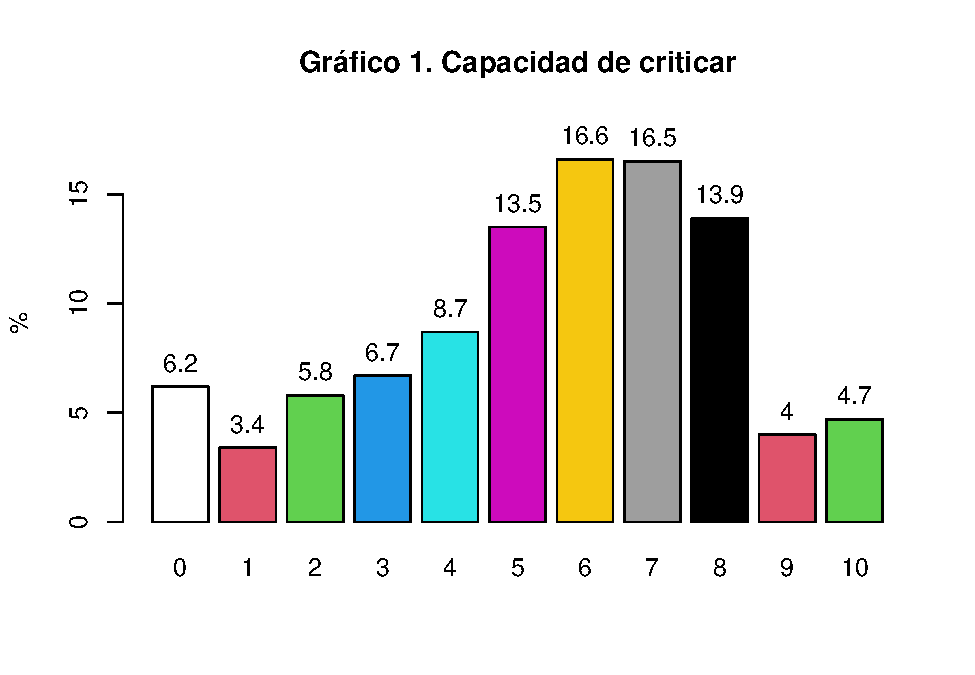
\includegraphics{libertadesItalia2022_files/figure-latex/dist-1.pdf}

\begin{Shaded}
\begin{Highlighting}[]
\CommentTok{\# Histograma}

\NormalTok{df\_ronda10SinNA }\OtherTok{\textless{}{-}}\NormalTok{ df\_ronda10[}\FunctionTok{complete.cases}\NormalTok{(}
\NormalTok{                                      df\_ronda10}\SpecialCharTok{$}\NormalTok{medcrgvc), ]}

\FunctionTok{hist}\NormalTok{(df\_ronda10}\SpecialCharTok{$}\NormalTok{medcrgvc, }\AttributeTok{col =} \StringTok{"lightblue"}\NormalTok{, }
                                          \AttributeTok{xlab =} \StringTok{"Capacidad de crítica (1{-}10)"}\NormalTok{, }
                                                     \AttributeTok{ylab =} \StringTok{"Frecuencia"}\NormalTok{,}
              \AttributeTok{main =} \StringTok{"Gráfico 2. Histograma de la Capacidad de criticar"}\NormalTok{)}

\FunctionTok{lines}\NormalTok{(}\FunctionTok{density}\NormalTok{(df\_ronda10SinNA}\SpecialCharTok{$}\NormalTok{medcrgvc), }\AttributeTok{col =} \StringTok{"red"}\NormalTok{, }\AttributeTok{lwd =} \DecValTok{1}\NormalTok{)}
\end{Highlighting}
\end{Shaded}

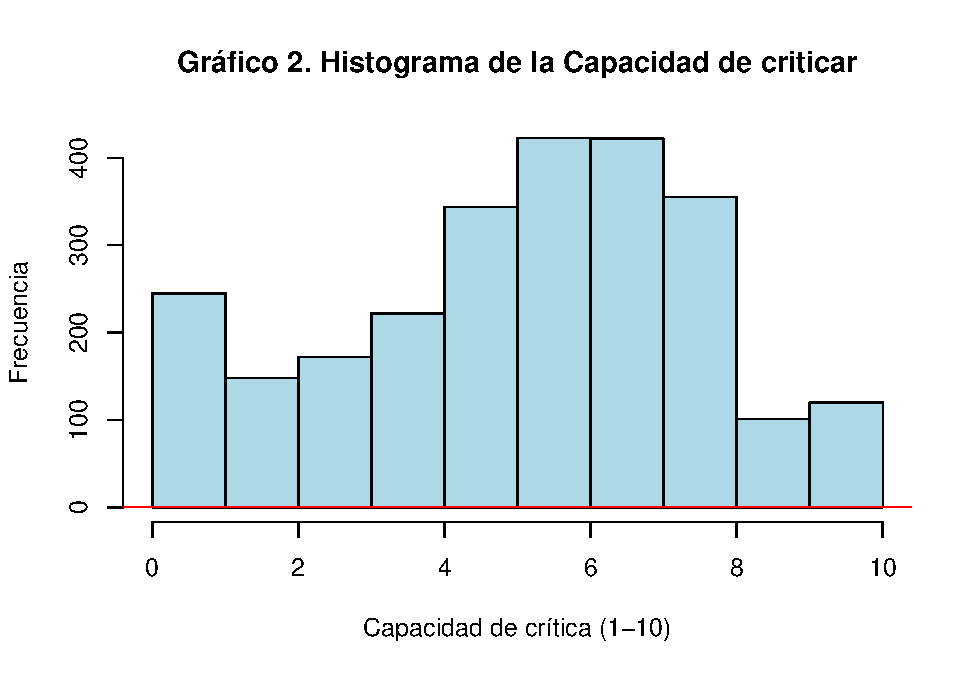
\includegraphics{libertadesItalia2022_files/figure-latex/histograma-1.pdf}

\newpage

\section{ANEXO 2. EJECUCIÓN DEL Rmd Y REPOSITORIO DE
FICHEROS}\label{anexo-2.-ejecuciuxf3n-del-rmd-y-repositorio-de-ficheros}

Para la ejecución del código R, está disponible el fichero ejecutable
Rmd y el fichero de datos \emph{sav} en el repositorio GitHub. En el
mismo repositorio se encuentra este PDF y un fichero HTML renderizados a
partir del Rmd.

El fichero \textbf{datosprac2.sav} debe ubicarse en una subcarpeta del
directorio de trabajo con nombre \emph{DATA}.

\begin{longtable}[]{@{}
  >{\centering\arraybackslash}p{(\columnwidth - 4\tabcolsep) * \real{0.2500}}
  >{\raggedright\arraybackslash}p{(\columnwidth - 4\tabcolsep) * \real{0.3500}}
  >{\raggedright\arraybackslash}p{(\columnwidth - 4\tabcolsep) * \real{0.4000}}@{}}
\toprule\noalign{}
\begin{minipage}[b]{\linewidth}\centering

\includegraphics[width=0.1\textwidth,height=\textheight]{../../recursos/iconohyperlink.jpg}
\end{minipage} & \begin{minipage}[b]{\linewidth}\raggedright
\end{minipage} & \begin{minipage}[b]{\linewidth}\raggedright
Enlace a GitHub
\end{minipage} \\
\midrule\noalign{}
\endhead
\bottomrule\noalign{}
\endlastfoot
\href{https://tofermos.github.io/cienciapoliticaygestionpublica/elecciones/italia/DATOS/datosprac2.sav}{
\includegraphics[width=0.1\textwidth,height=\textheight]{../../recursos/iconosav.png}}
& Fichero de datos tipo sav &
\href{https://tofermos.github.io/cienciapoliticaygestionpublica/elecciones/italia/DATOS/datosprac2.sav}{datosprac2.sav} \\
\href{https://tofermos.github.io/cienciapoliticaygestionpublica/elecciones/italia/libertadesItalia2022.Rmd}{
\includegraphics[width=0.1\textwidth,height=\textheight]{../../recursos/rmarkdown.png}}
& Fichero Rmd &
\href{https://tofermos.github.io/cienciapoliticaygestionpublica/elecciones/italia/libertadesItalia2022.Rmd}{libertadesItalia2022.Rmd} \\
\href{https://tofermos.github.io/cienciapoliticaygestionpublica/elecciones/italia/libertadesItalia2022.html}{
\includegraphics[width=0.1\textwidth,height=\textheight]{../../recursos/iconohtml.png}}
& Fichero HTML &
\href{https://tofermos.github.io/cienciapoliticaygestionpublica/elecciones/italia/libertadesItalia2022.html}{libertadesItalia2022.html} \\
\href{https://tofermos.github.io/cienciapoliticaygestionpublica/elecciones/italia/libertadesItalia2022.pdf}{
\includegraphics[width=0.1\textwidth,height=\textheight]{../../recursos/iconopdf.png}}
& Fichero PDF &
\href{https://tofermos.github.io/cienciapoliticaygestionpublica/elecciones/italia/libertadesItalia2022.pdf}{libertadesItalia.pdf} \\
\href{https://tofermos.github.io/cienciapoliticaygestionpublica/}{
\includegraphics[width=0.2\textwidth,height=\textheight]{../../recursos/iconogithub.png}}
& &
\href{https://tofermos.github.io/cienciapoliticaygestionpublica/}{Repositorio
tofermos} \\
\end{longtable}

\end{document}
